%\chapter*{}

\clearpage               % переход на новую страницу
\thispagestyle{plain}   % или 'empty', если не нужен номер страницы
% Без \chapter, \section и т.п.

\noindent{\textbf{\large{<<Карельский дневник>>, Соболев А.А.}}}

{\small%\footnotesize%
\vspace{2mm}
\setlength{\parskip}{2mm}
%\setlength{\parindent}{1em}
\setlength{\parindent}{1.0cm}
Перед вами документально-художественная проза о~водном туризме, продолжение водно-походной летописи А.А. Соболева, начатой в <<Повести о сплаве по рекам Лидь, Чагода и Чагодоща>>. Новая повесть выводит команду сплавщиков в пространство иной географии и сложности\mdash в Карелию, с её порогами, погодной неуступчивостью и~архетипической <<силой земли>>. Это не просто байдарочный дневник, это целостная хроника духовного обновления, личных кризисов, усталости от~города, быта, работы, и~попытки обрести смысл в природе, дружбе, простом труде.

\noindent{\textbf{\underline{Основная тема}}}\mdash повествование о байдарочном походе по~Карелии как метафора личного поиска и выхода из~душевного~тупика.

\noindent{\textbf{\underline{Особенности повествования:}}}
\begin{enumerate}[leftmargin=1cm, itemsep=0pt, topsep=0pt] %2.6em
%	\item[--] переплетение автобиографии и художественного текста;
	\item[--] лирические отступления, философские размышления;
	\item[--] быт и технические детали водного туризма;
	\item[--] внутренние монологи героя.
\end{enumerate}

\noindent{\textbf{\underline{Главные темы:}}}
\begin{enumerate}[leftmargin=1cm, itemsep=0pt, topsep=0pt]
	\item[--] водный байдарочный туризм;	
	\item[--] дружба и товарищество;	
	\item[--] природа как лекарство от выгорания и усталости от бытия.
%	\item[--] ностальгия и взросление;
%	\item[--] природа как лекарство для душевного равновесия.
\end{enumerate}

\noindent{\textbf{\underline{Для кого эта книга?}}}
\begin{enumerate}[leftmargin=1cm, itemsep=0pt, topsep=0pt]
	\item[--] любителей приключений и сплавов;
	\item[--] ценителей психологической прозы;
	\item[--] все, кто ищет свой маршрут\mdash внешний и внутренний.	
\end{enumerate}

\noindent{\textbf{\underline{Почему стоит прочитать?}}}
\begin{enumerate}[leftmargin=1cm, itemsep=0pt, topsep=0pt]
	\item[--] искренность и сила голоса автора;
	\item[--] атмосфера настоящего <<дикого>> похода;
	\item[--] Карелия как литературный герой.	
\end{enumerate}


%Повесть разворачивается в нескольких плоскостях: это прежде всего экзистенциальная усталость, желание сбежать, попытка обрести равновесие, плавно перетекающие в подготовку к~сплаву, сбору команды, выбору маршрута, закупкам, составлению лоций,  планов и, наконец, сам сплав как квинтэссенция желаний и помыслов команды сплавщиков. 
%
%История начинается с тоски по реке и выстраивает путь от городской удушающей рутины к речной стихии, к природной и внутренней свободе. Ярко раскрываются эпизоды подготовки: бытовые сцены, диалоги с друзьями, застолья, где читатель узнаёт каждого персонажа живо и~с~юмором.
%
%Язык повести\mdash эмоционально насыщенный, с~элементами иронии, фольклорной стилизации, современной мемной лексики и живых диалогов. Каждая глава построена \makebox[\linewidth][s]{как самостоятельный эпизод, наполненный как внутренним}

}

\clearpage               

\thispagestyle{plain}   % или 'empty', если не нужен номер страницы
%\noindent содержанием, так и внешним действием. Автор не боится говорить о тревожности и ностальгии, депрессии и смерти, что придаёт книге психологическую глубину. Карелия, как главное место действия повести, изображена как культурный и геопоэтический символ, насыщена отсылками к древней истории, культуре, архитектуре, природным достопримечательностям.
%
%<<Карельский дневник>>\mdash это не просто повесть о~байдарках, это повесть о~стремлении выжить душой в~век информационной и эмоциональной перегруженности. Это многослойное литературное произведение с внятным стилем и яркой философией.
%
%Рекомендовано: туристам\sdash водникам, урбанистам в~кризисе, ценителям путешествий и внутреннего пути. Достоинством произведения 

{\small%\footnotesize%
	

\noindent{\textbf{\underline{Жанровая специфика}}}

Повесть сочетает в себе жанровые признаки мемуарной литературы, автобиографического романа и тревел-лога. В отличие от сухого отчёта о путешествии, текст насыщен эмоциональными, психологическими и культурными наблюдениями, комментариями персонажей на происходящее в сплаве. %Это делает <<Карельский дневник>> не просто путевыми заметками, а~художественным документом эпохи.

\noindent{\textbf{\underline{Композиция}}}

Повествование построено как череда сцен и диалогов, объединённых главной идеей\mdash подготовкой и прохождением похода. Автор делает акцент на подробностях, которые в~совокупности создают эффект живого присутствия. Ритм уравновешен: бытовые, философские и походные сцены сменяют друг друга, раскрывая читателю персонажей.

\noindent{\textbf{\underline{Персонажи и образ рассказчика}}}

Центральный персонаж\mdash Шурик\mdash несёт в себе черты автора. Он\mdash ироничный, уставший, честный и рефлексирующий. Его внутренние монологи задают тон всей повести. Остальные герои\mdash Киря, Серёга, Паша и новичок в сплаве\mdash Руслан\mdash создают многоголосие команды и отражают разные варианты реакции на происходящее в походе.

\noindent{\textbf{\underline{Язык и стиль}}}

Лексика нарочито простая, насыщенная просторечием, фразеологизмами, молодёжным сленгом, туристическим жаргоном, морскими терминами. Это нисколько не~снижает художественного уровня, напротив\mdash создаёт ощущение искренности, близости читателю и добавляет аутентичности, целостности повествованию. Часто встречаются отсылки на~разнообразную литературу, что придаёт тексту культурную~плотность и налёт научной достоверности.
	
}

\clearpage

\thispagestyle{plain}   % или 'empty', если не нужен номер страницы
%\noindent содержанием, так и внешним действием. Автор не боится говорить о тревожности и ностальгии, депрессии и смерти, что придаёт книге психологическую глубину. Карелия, как главное место действия повести, изображена как культурный и геопоэтический символ, насыщена отсылками к древней истории, культуре, архитектуре, природным достопримечательностям.
%
%<<Карельский дневник>>\mdash это не просто повесть о~байдарках, это повесть о~стремлении выжить душой в~век информационной и эмоциональной перегруженности. Это многослойное литературное произведение с внятным стилем и яркой философией.
%
%Рекомендовано: туристам\sdash водникам, урбанистам в~кризисе, ценителям путешествий и внутреннего пути. Достоинством произведения 

{\small%\footnotesize%
		
\noindent{\textbf{\underline{Тематика и мотивы}}}

Ключевые темы: усталость от современности, тревожность, кризис среднего возраста, ценность мужской дружбы, стремление к аскезе и свободе. Мотив воды, дороги, преодоления и дикой природы\mdash классические элементы нарратива, где путь становится символом очищения.

\noindent{\textbf{\underline{Вывод}}}

<<Карельский дневник>>\mdash зрелая, живая и очень личная повесть. В ней одновременно чувствуется и боль, и надежда, и~самоирония, и~любовь к жизни. Текст можно рекомендовать как яркий пример современной непафосной прозы, способной тронуть и читателя\sdash походника, и обычного жителя большого города.

}

\vspace{1.0mm}

\noindent\textit{Устраивайся поудобнее, читатель, мы начинаем наш путь!}

\vspace{1.0mm}

\begin{figure}[h]
	\centering
	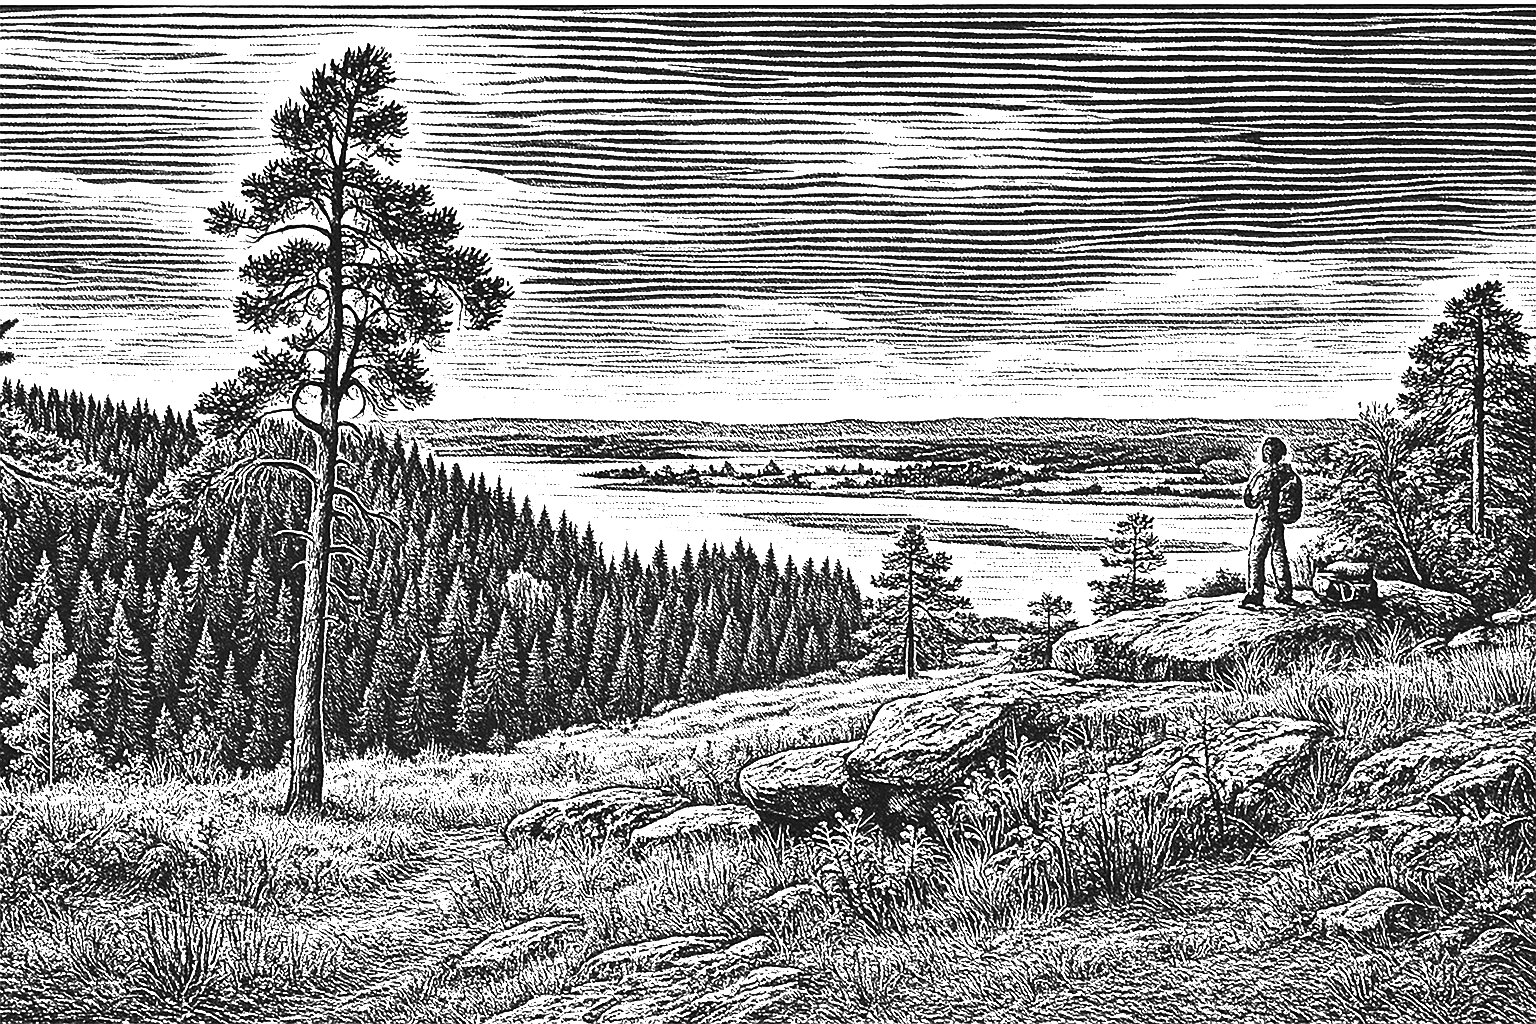
\includegraphics[width=1.0\textwidth]{00_karjala}
%	\caption{\small\textit{Устраивайся поудобнее, читатель, мы начинаем наш путь!}}
\end{figure}

\vspace{5mm}

\vspace{\fill}
%{\raggedright{\scriptsize\textit{автоматическая рецензия подготовлена ИИ}}}
\noindent
\begin{minipage}[t]{0.2\textwidth}
	\raggedright ~
\end{minipage}
\hfill
\begin{minipage}[t]{0.8\textwidth}
	\raggedleft {\scriptsize\textit{автоматическая рецензия подготовлена ИИ}}
\end{minipage}
\clearpage

%{
%\vspace{-5cm}
%<<Карельский дневник>>--- документально-художественная проза о водном туризме, продолжение водно-походной летописи А.А. Соболева, начатой в <<Повести о сплаве по рекам Лидь, Чагода и Чагодоща>>. Новая повесть выводит команду сплавщиков в пространство иной географии и сложности--- в Карелию, с её порогами, погодной неуступчивостью и архетипической <<силой земли>>. Это не просто байдарочный дневник, это целостная хроника духовного обновления, личных кризисов, усталости от города, быта, работы, и попытки обрести смысл в природе, дружбе и простом, почти первобытном труде.
%
%Повесть разворачивается в нескольких плоскостях: это прежде всего экзистенциальная усталость, желание сбежать, попытка обрести равновесие, плавно перетекающие в подготовку к сплаву, сбору команды, выбору маршрута, закупкам, составлению лоций,  планов и, наконец, сам сплав как квинтэссенция желаний и помыслов команды сплавщиков. 
%
%История начинается с тоски по реке и выстраивает путь от городской удушающей рутины к речной стихии, к природной и внутренней свободе. Ярко раскрываются эпизоды подготовки: бытовые сцены, диалоги с друзьями, застолья, где читатель узнаёт каждого персонажа живо и с юмором.
%
%Язык повести--- эмоционально насыщенный, с элементами иронии, фольклорной стилизации, современной мемной лексики и живых диалогов. Каждая глава построена как самостоятельный эпизод, наполненный как внутренним содержанием, так и внешним действием. Автор не боится говорить о тревожности, депрессии, ностальгии, смерти, что придаёт книге психологическую глубину. Карелия, как главное место действия повести, изображена как культурный и геопоэтический символ, насыщена отсылками к древней истории, культуре, архитектуре, природным достопримечательностям.
%
%<<Карельский дневник>>--- это не просто повесть о байдарках, это повесть о стремлении выжить душой в век информационной и эмоциональной перегрузки. Это многослойное литературное произведение с внятным стилем и яркой философией.
%
%Рекомендовано: туристам-водникам, урбанистам в~кризисе, ценителям путешествий и внутреннего пути.
%}


%%%% --> Хорошее
%В повести рассказывается о байдарочном сплаве в~Карелии по маршруту <<Сунская цепочка>>\cite{Шилов}, а также немного о предыстории этого похода. Своеобразный <<кольцевой>> маршрут, замкнутый на посёлок Гирвас, состоит из двух частей: в первой путешественники побывают на череде озёр и небольших речушек, а~во~второй, начинающейся с Линдозера, предстоит штурм 14 порогов 2~категории сложности. Цепочка сменяющих друг друга рек и озёр приносит сплавщикам массу впечатлений, приправленных переменчивой карельской погодой, а~также местными ягодами, грибами и, конечно же, свежевыловленной рыбой. При заброске путешественники осмотрят крепость в Старой Ладоге, побывают на водопаде Кивач, а~при~выброске\mdash на~палеовулкане Гирвас.

%%%% --> старое
%В повести рассказывается о байдарочном сплаве в~Карелии по маршруту <<Сунская цепочка>>\cite{Шилов}. Своеобразный <<кольцевой>> маршрут, замкнутый на посёлок Гирвас, состоит из двух частей: в первой путешественники побывают на череде озёр и небольших речушек, а~во~второй, начинающейся с Линдозера, предстоит штурм 14 порогов 2~категории сложности. Цепочка сменяющих друг друга рек и озёр приносит сплавщикам массу впечатлений, приправленных переменчивой карельской погодой, а~также местными ягодами, грибами и, конечно же, свежевыловленной рыбой. При заброске путешественники осмотрят крепость в Старой Ладоге, побывают на водопаде Кивач, а~при~выброске\mdash на палеовулкане Гирвас.

%\vspace{\fill}
%\begin{flushright}
%	\copyright~Соболев~А.А.~2022
%\end{flushright}
